\documentclass[10pt,xcolor={dvipsnames}]{beamer}
\usetheme[
%%% option passed to the outer theme
%    progressstyle=fixedCircCnt,   % fixedCircCnt, movingCircCnt (moving is deault)
  ]{Feather}
  
% If you want to change the colors of the various elements in the theme, edit and uncomment the following lines

% Change the bar colors:
\setbeamercolor{Feather}{fg=NavyBlue!20,bg=NavyBlue}

% Change the color of the structural elements:
\setbeamercolor{structure}{fg=NavyBlue}

% Change the frame title text color:
\setbeamercolor{frametitle}{fg=black!5}

% Change the normal text colors:
\setbeamercolor{normal text}{fg=black!75,bg=gray!5}

%% Change the block title colors
\setbeamercolor{block title}{use=Feather,bg=Feather.fg, fg=black!90} 


% Change the logo in the upper right circle:
%\renewcommand{\logofile}{example-grid-100x100pt} 
%% This is an image that comes with the LaTeX installation
% Adjust scale of the logo w.r.t. the circle; default is 0.875
% \renewcommand{\logoscale}{0.55}

% Change the background image on the title and final page.
% It stretches to fill the entire frame!
% \renewcommand{\backgroundfile}{example-grid-100x100pt}

%-------------------------------------------------------
% INCLUDE PACKAGES
%-------------------------------------------------------

\usepackage[utf8]{inputenc}
\usepackage[english]{babel}
\usepackage[T1]{fontenc}
% \usepackage{helvet}

%% Load different font packages to use different fonts
%% e.g. using Linux Libertine, Linux Biolinum and Inconsolata
% \usepackage{libertine}
% \usepackage{zi4}

%% e.g. using Venturis ADF Serif and Sans
% \usepackage{venturis}

%-------------------------------------------------------
% DEFFINING AND REDEFINING COMMANDS
%-------------------------------------------------------

% colored hyperlinks
\newcommand{\chref}[2]{
  \href{#1}{{\usebeamercolor[bg]{Feather}#2}}
}

%-------------------------------------------------------
% INFORMATION IN THE TITLE PAGE
%-------------------------------------------------------

\title[Fund Computación] % [] is optional - is placed on the bottom of the sidebar on every slide
{ % is placed on the title page
      \Large{\textbf{Fundamentación en computación}}
}

\subtitle[Clase 2]
{
      \textbf{Las partes del computador}
}

\author[Julián Calle]
{      Julián Calle \\
      {\ttfamily julian.callem@udea.edu.co} \\ \vspace{0.5cm}
      Clase 2
}

\institute[UdeA]
{%
\begin{columns}
\begin{column}{3cm}

\includegraphics[scale=0.045]{Feathergraphics/2-2} 
\end{column}
\begin{column}{6cm} 
Instituto de física\\
Facultad de ciencias exactas y naturales \\
Universidad de Antioquia
\end{column} \end{columns}
}

\date{\today}

%-------------------------------------------------------
% THE BODY OF THE PRESENTATION
%-------------------------------------------------------

\begin{document}

%-------------------------------------------------------
% THE TITLEPAGE
%-------------------------------------------------------

{\1
\begin{frame}[plain,noframenumbering]
  \titlepage
\end{frame}}


\begin{frame}{Content}{}
\tableofcontents
\end{frame}

\begin{frame}{PC}
\begin{center}
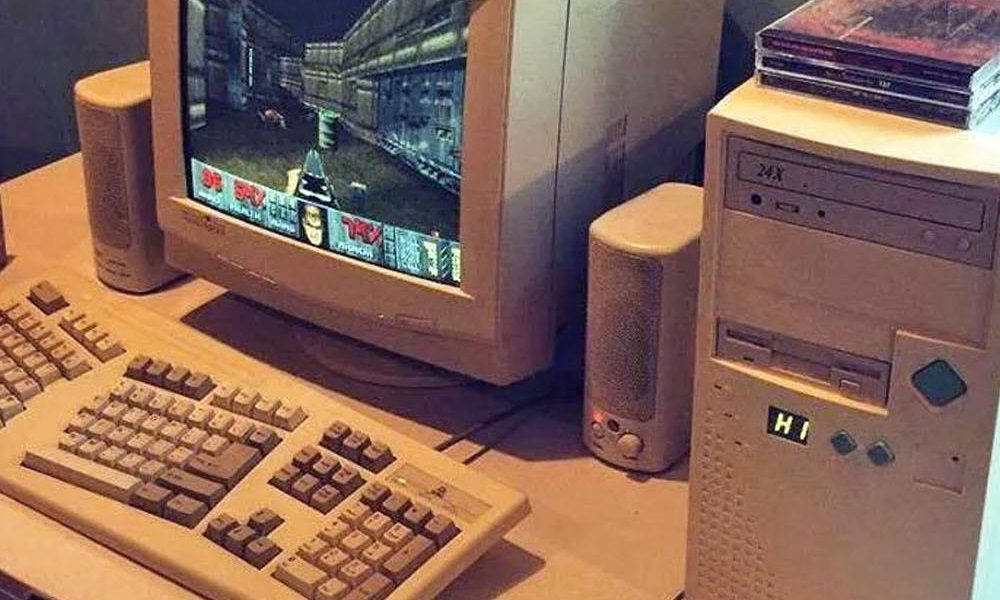
\includegraphics[scale=0.15]{Figures/pcRetro}
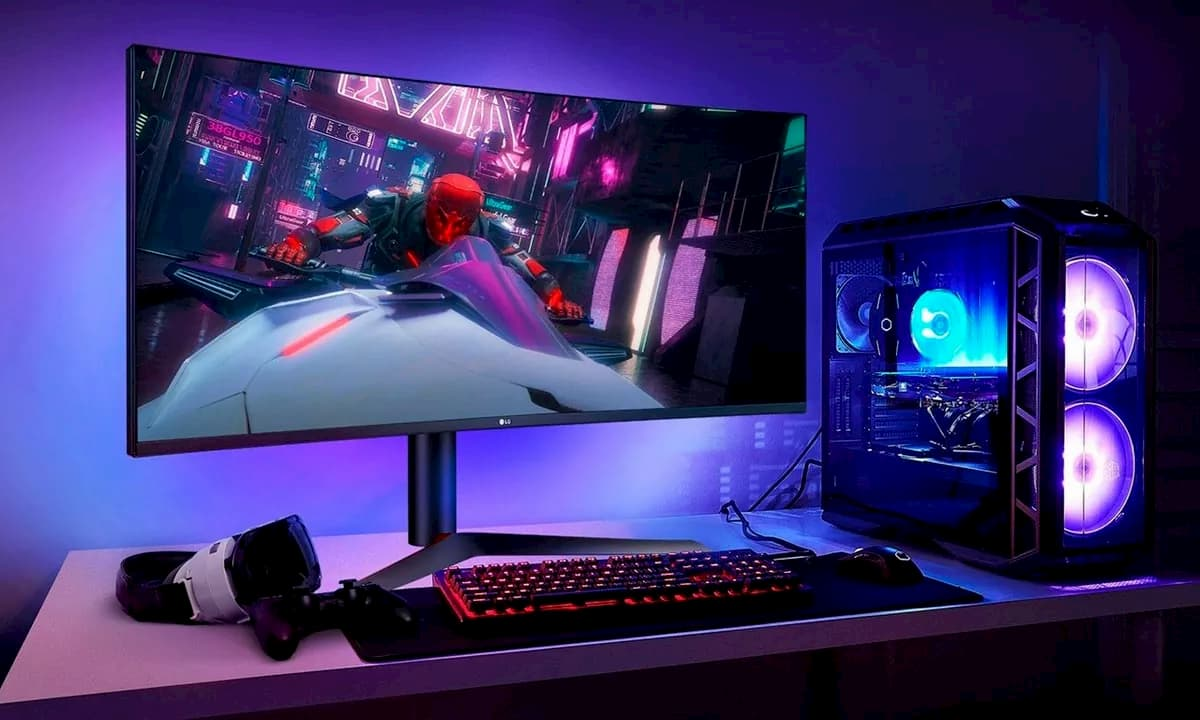
\includegraphics[scale=0.13]{Figures/pc}
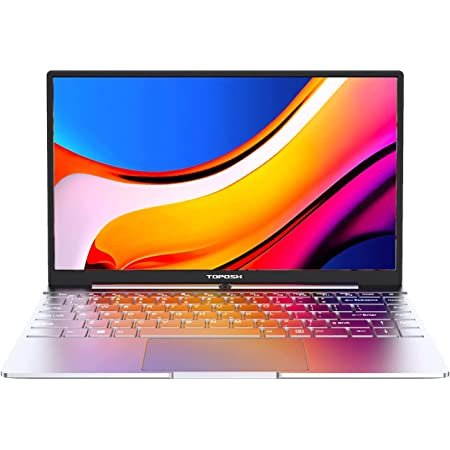
\includegraphics[scale=0.25]{Figures/Portatil}
\end{center}
\end{frame}

\begin{frame}{Cerebro}
\begin{center}
\only<1>{
\includegraphics[scale=0.6]{Figures/cerevro}}
\only<2>{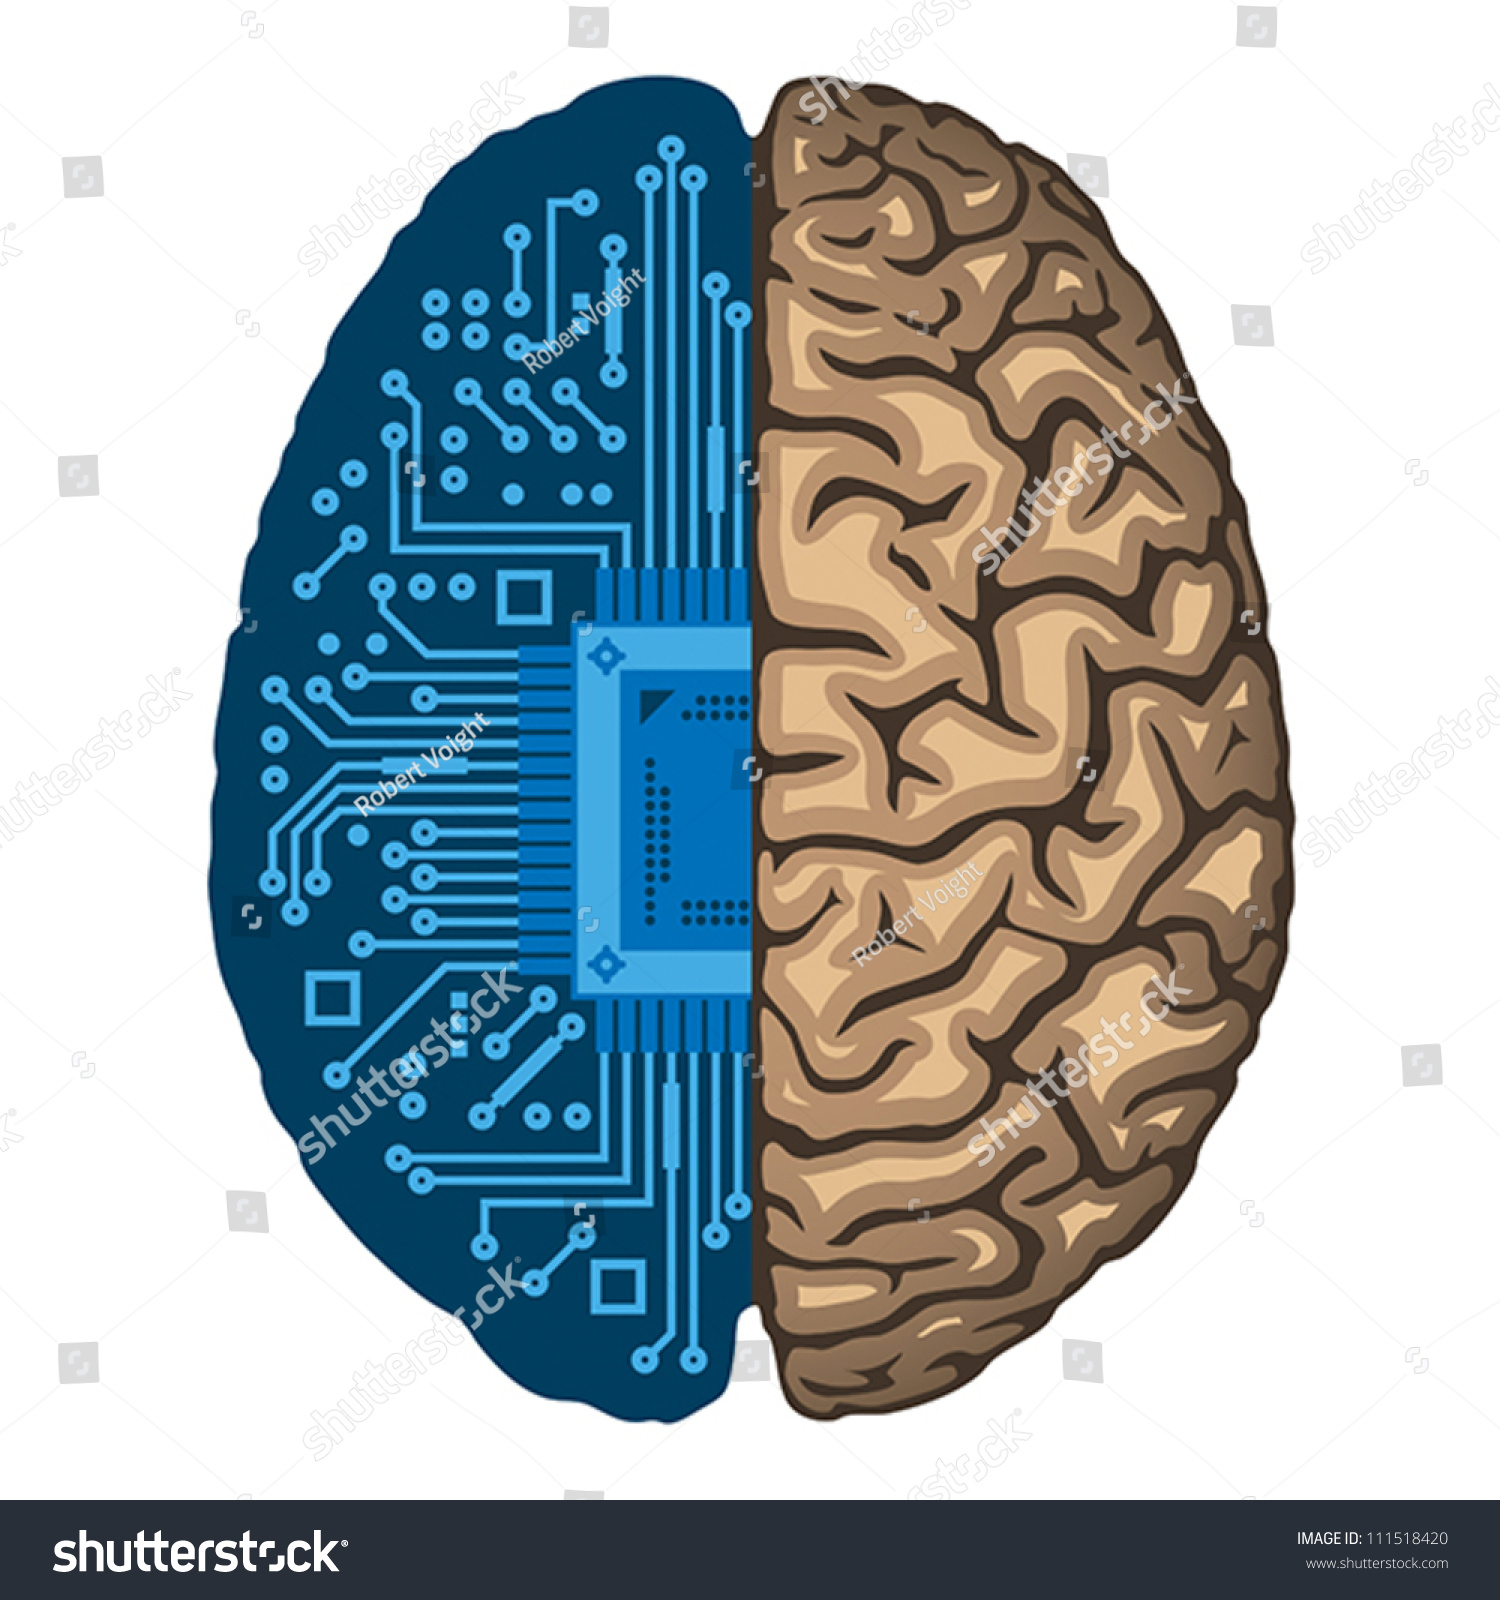
\includegraphics[scale=0.5]{Figures/cerebro}}
\end{center}
\end{frame}

\begin{frame}
\begin{center}
\Huge{\textcolor{blue}{Maquina Universal de Turing}}
\end{center}
\end{frame}

\begin{frame}{Maquina de Turing}
\begin{center}
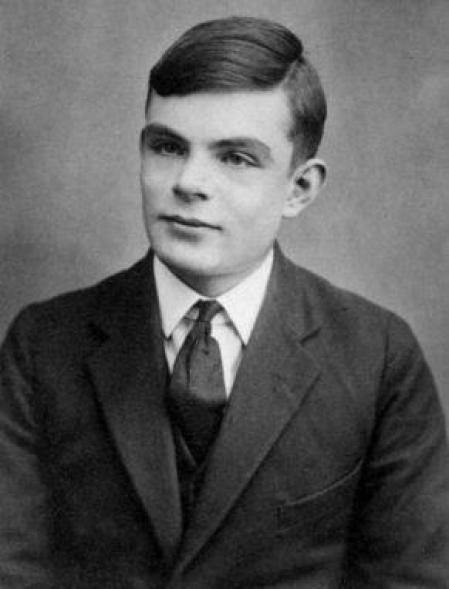
\includegraphics[scale=0.4]{Figures/Turing} \\ \pause
\url{https://turingmachine.io/}
\end{center}
\end{frame}

\begin{frame}
\begin{center}

\includegraphics[scale=0.5]{Figures/estamuerto}
\end{center}
\end{frame}

\begin{frame}
\begin{center}

\includegraphics[scale=0.7]{Figures/Shrek1}
\end{center}
\end{frame}

\section{CPU}
\begin{frame}
\begin{center}
\Huge{\textcolor{blue}{CPU}}
\end{center}
\end{frame}

\begin{frame}{El cerebro del pc}
\begin{center}
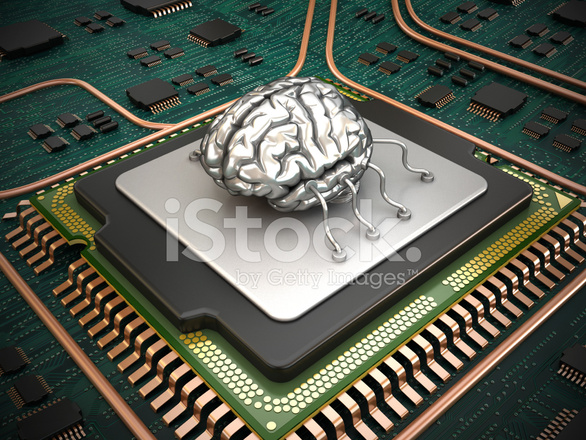
\includegraphics[scale=0.4]{Figures/cpuCerebro}
\end{center}
\end{frame}

\begin{frame}{CPU}
\begin{center}
\only<2>{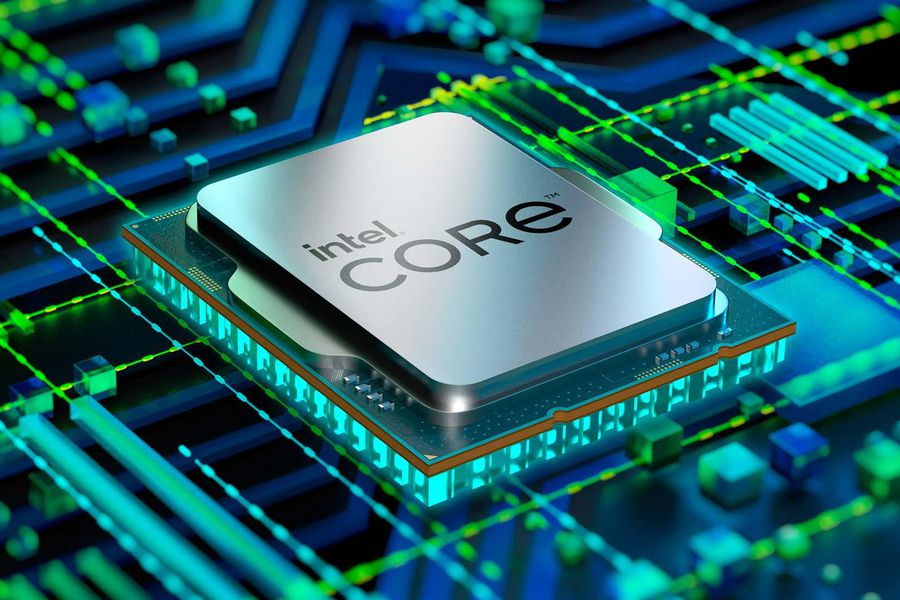
\includegraphics[scale=0.3]{Figures/Procesador1}}
\only<3>{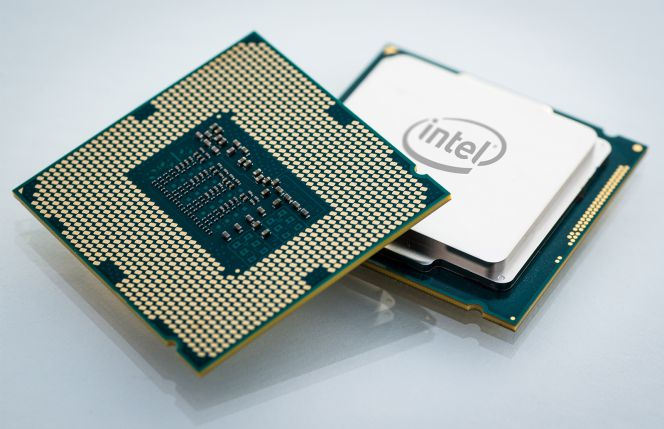
\includegraphics[scale=0.4]{Figures/procesador}}
\only<4>{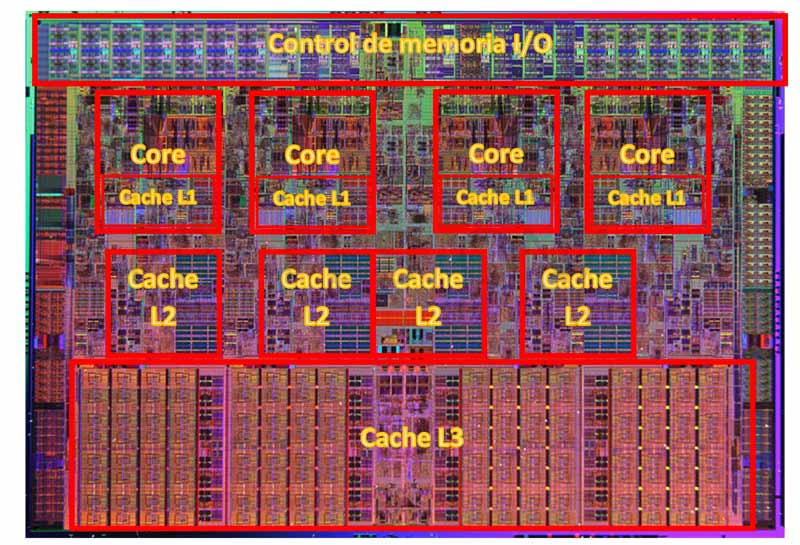
\includegraphics[scale=0.35]{Figures/Procesador}}
\only<5>{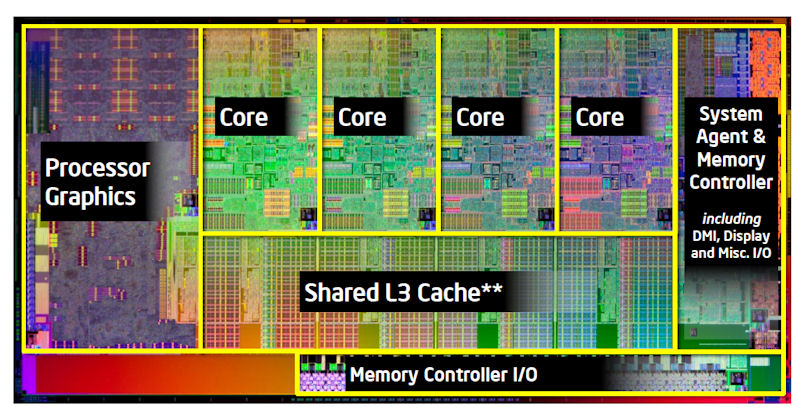
\includegraphics[scale=0.5]{Figures/ProcesadorInt}}
\end{center}
\end{frame}


\begin{frame}
\begin{center}
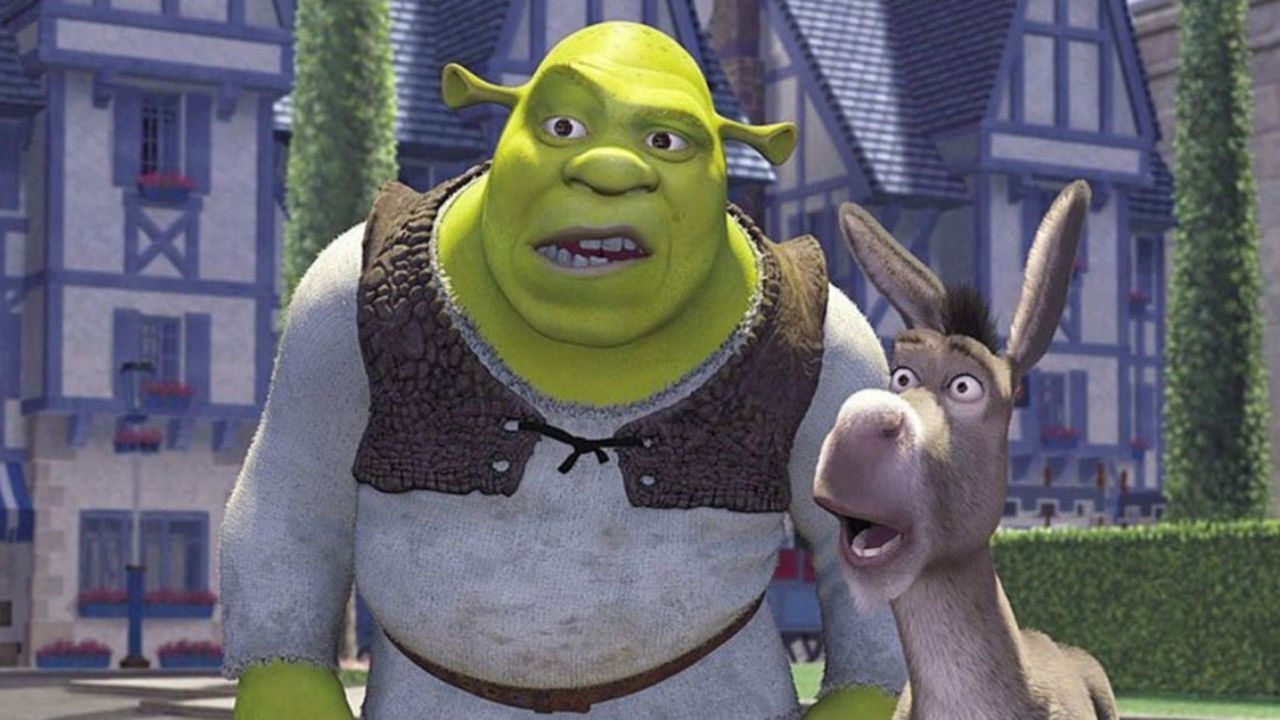
\includegraphics[scale=0.25]{Figures/Shrek3}
\end{center}
\end{frame}

\section{Memorias}
\begin{frame}
\begin{center}
\Huge{\textcolor{blue}{Memorias}}
\end{center}
\end{frame}

\begin{frame}{Almacenamiento}
\begin{center}
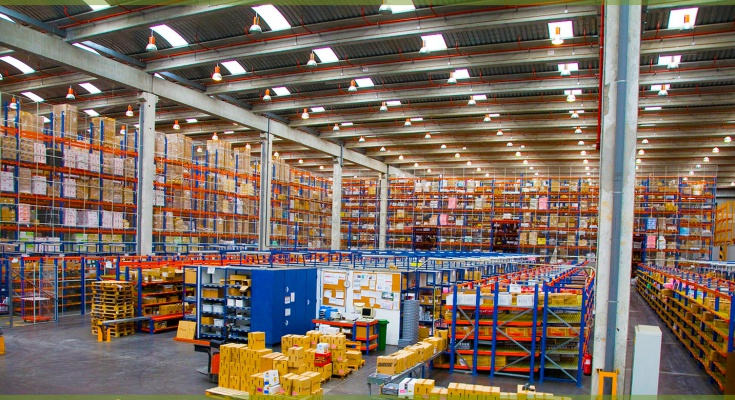
\includegraphics[scale=0.4]{Figures/Bodega}
\end{center}
\end{frame}

\begin{frame}
\begin{center}
\Huge{\textcolor{blue}{Unidad de almacenamiento}}
\end{center}
\end{frame}

\begin{frame}{HDD}
\begin{center}
\only<2->{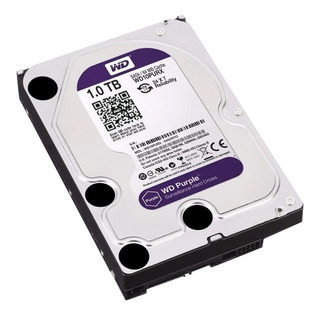
\includegraphics[scale=0.4]{Figures/hhd1}}
\only<3>{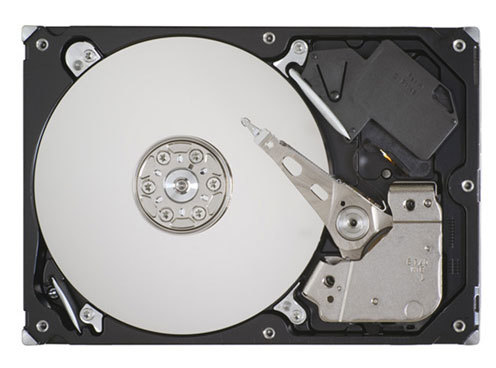
\includegraphics[scale=0.4]{Figures/hhd}}
\end{center}
\end{frame}

\begin{frame}{SSD Sata}
\begin{center}
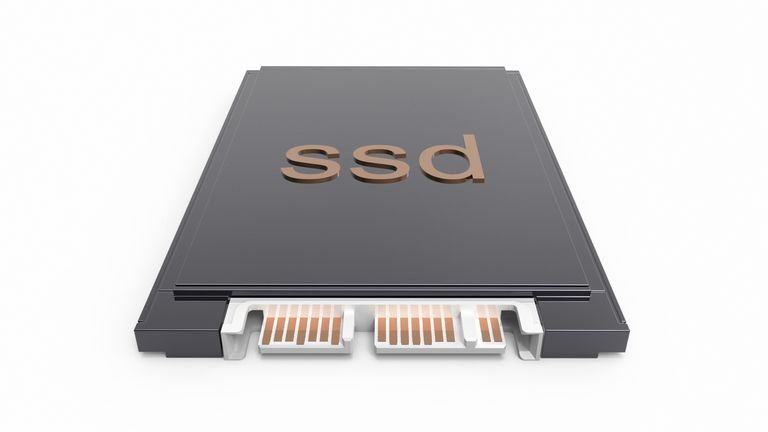
\includegraphics[scale=0.4]{Figures/ssdsata}
\end{center}
\end{frame}

\begin{frame}{SSD M.2}
\begin{center}
\only<2>{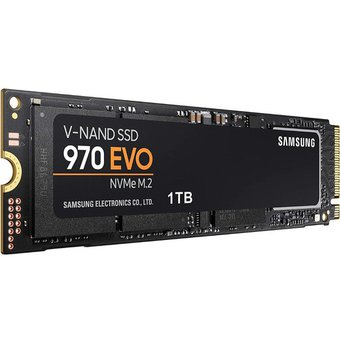
\includegraphics[scale=0.4]{Figures/ssdm2}}
\only<3>{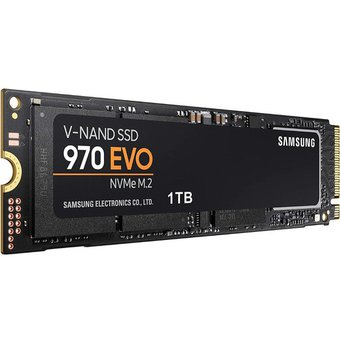
\includegraphics[scale=0.2]{Figures/ssdm2}}
\only<3>{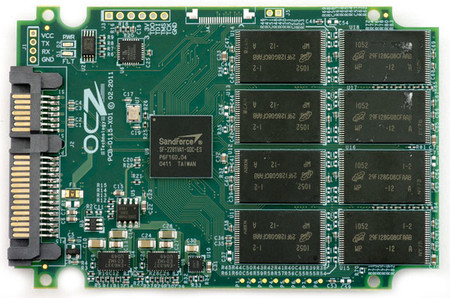
\includegraphics[scale=0.4]{Figures/ssd}}
\end{center}
\end{frame}

\begin{frame}{¿Cuál es mejor?}
\begin{center}
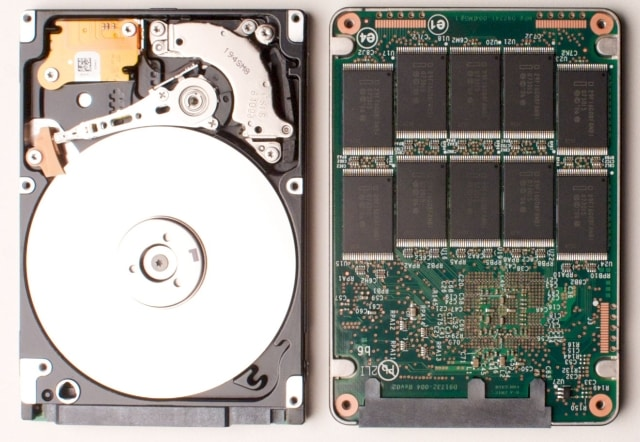
\includegraphics[scale=0.4]{Figures/HHD-o-SSD}
\end{center}
\end{frame}


\begin{frame}
\begin{center}

\includegraphics[scale=0.7]{Figures/Patricio}
\end{center}
\end{frame}

\begin{frame}
\begin{center}
\Huge{\textcolor{blue}{RAM}} \\ \pause
\Large{Random Access Memory}
\end{center}
\end{frame}

\begin{frame}{RAM}
\begin{center}
\only<2>{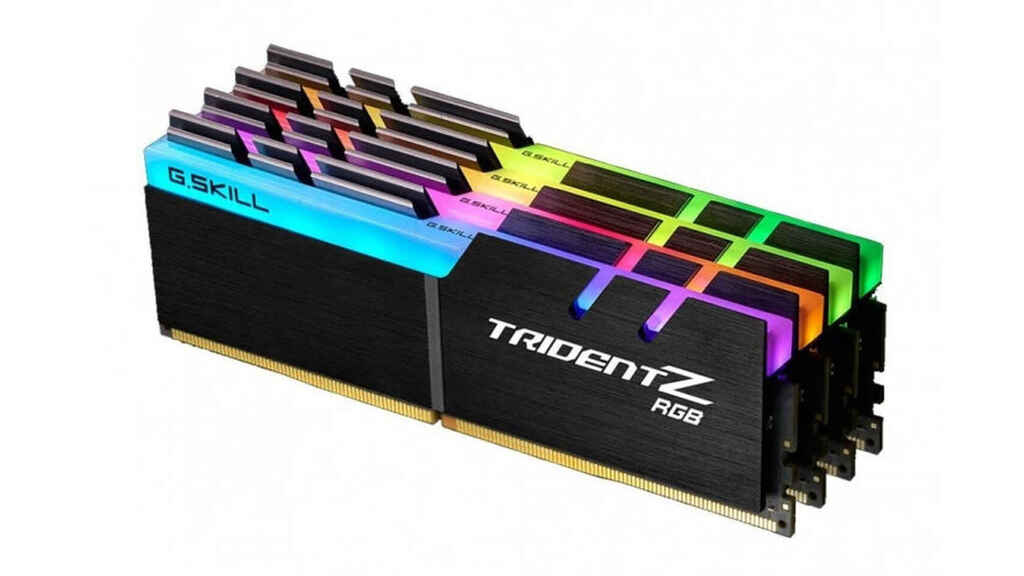
\includegraphics[scale=0.8]{Figures/RAM1}}
\only<3>{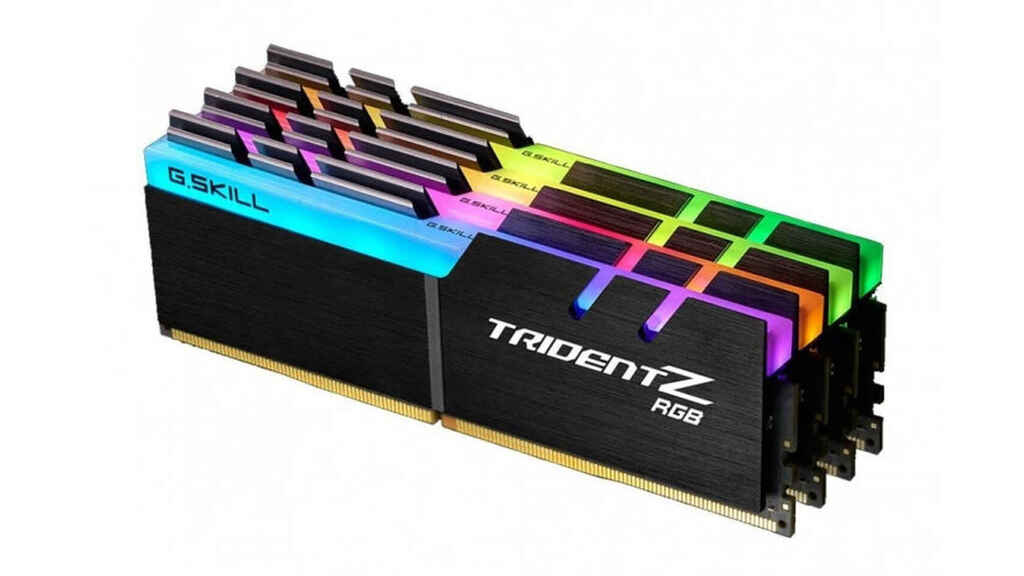
\includegraphics[scale=0.4]{Figures/RAM1}}
\only<3>{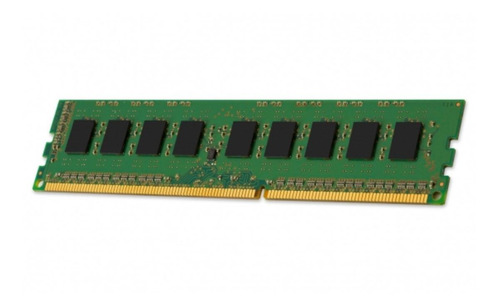
\includegraphics[scale=0.5]{Figures/RAM}}
\end{center}
\end{frame}

\begin{frame}{¿Todos los números tienen nombre?}
\begin{center}
\only<2>{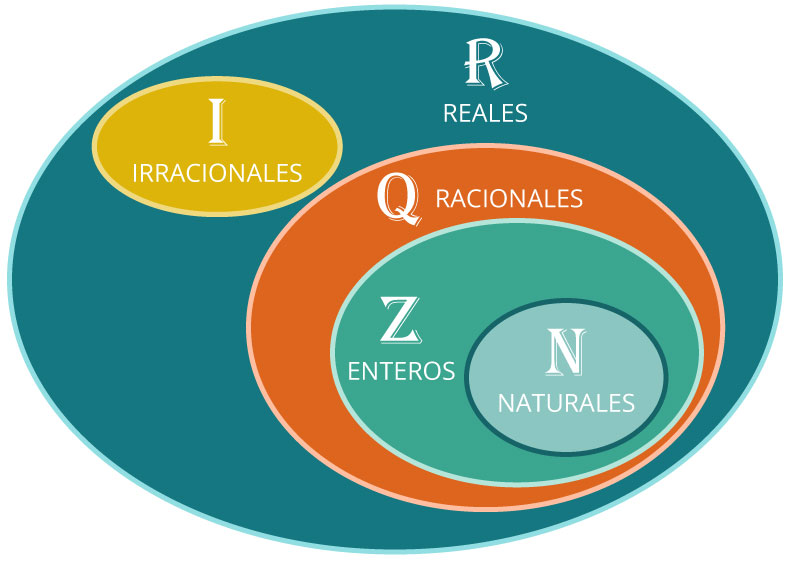
\includegraphics[scale=0.3]{Figures/numeros}}
\only<3>{
\includegraphics[scale=0.5]{Figures/Infinito}}
\only<4>{
\includegraphics[scale=0.5]{Figures/Infinito1}}
\only<5-6>{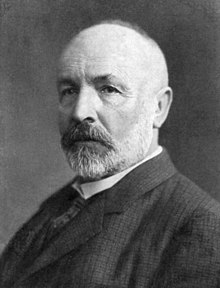
\includegraphics[scale=0.5]{Figures/Cantor} \\}
\only<6>{
\includegraphics[scale=0.2]{Figures/tinder}}
\only<7>{
\includegraphics[scale=0.25]{Figures/infinitos2}}
\only<8>{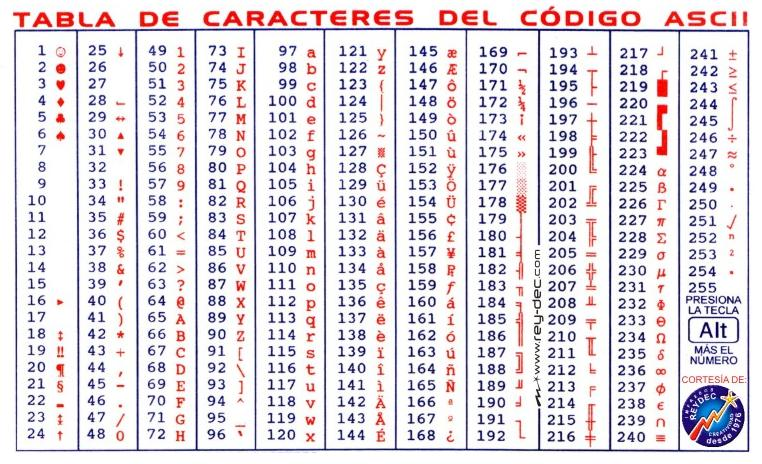
\includegraphics[scale=0.5]{Figures/ascii}}
\end{center}
\end{frame}

\section{Placa base}
\begin{frame}
\begin{center}
\Huge{\textcolor{blue}{Placa base}}
\end{center}
\end{frame}

\begin{frame}{Placa base}
\begin{center}
\only<2>{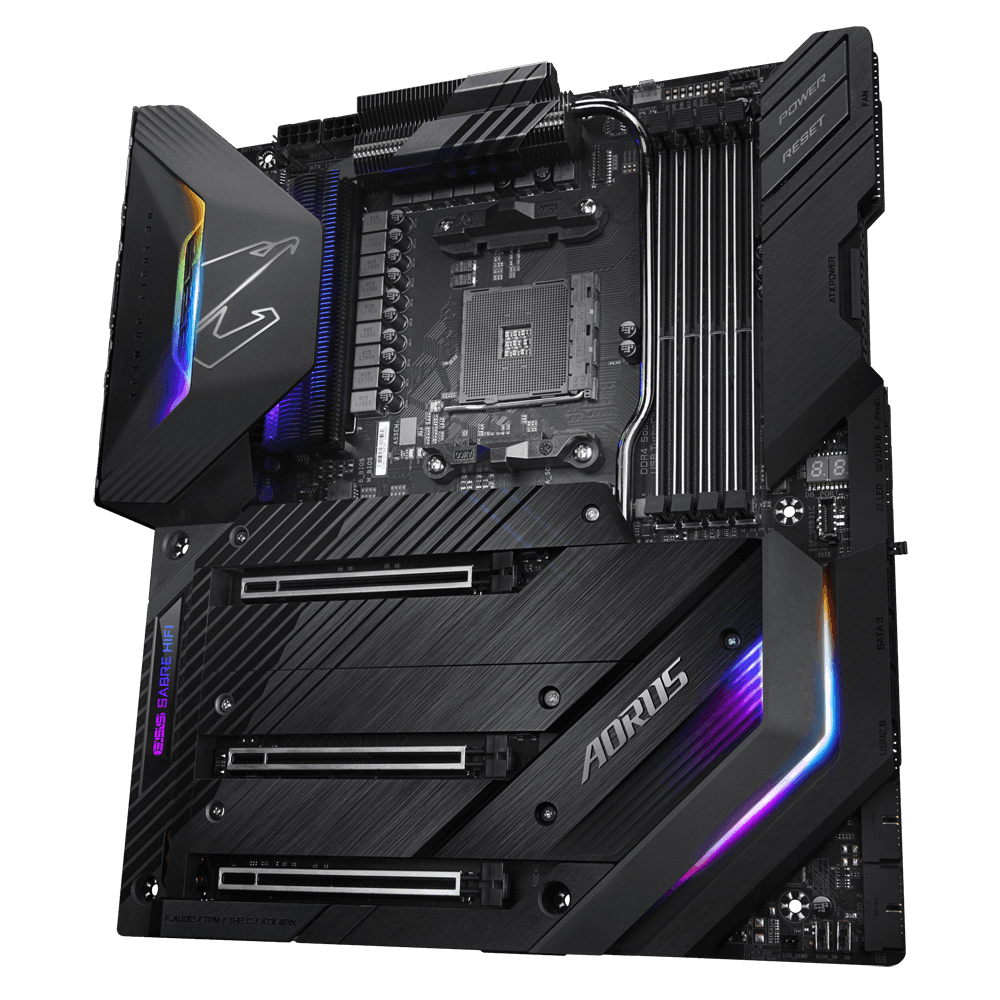
\includegraphics[scale=0.2]{Figures/Placa}}
\only<3>{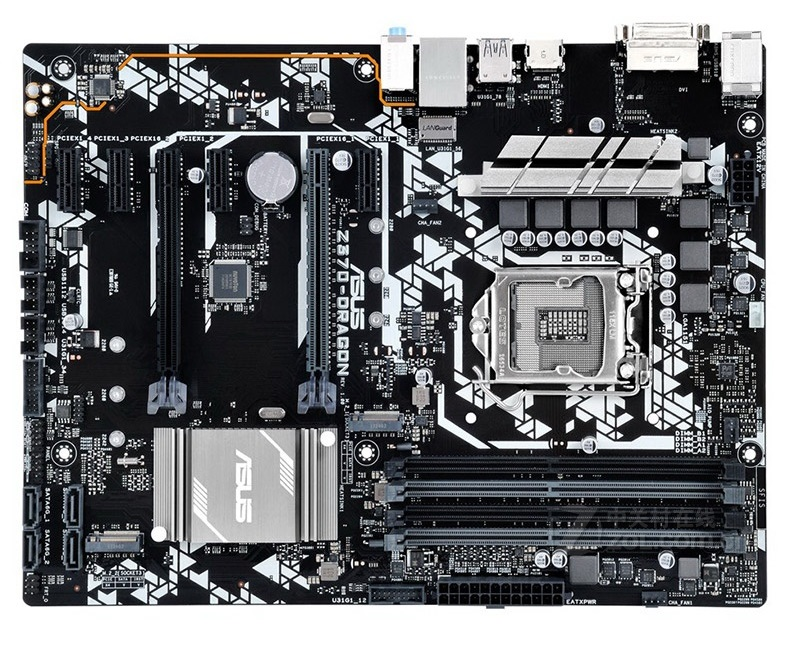
\includegraphics[scale=0.43]{Figures/Placa1}}
\end{center}
\end{frame}

\begin{frame}
\begin{center}
\Large{\textcolor{red}{Las partes de la placa base son las siguientes:}} \\ \pause

\includegraphics[scale=0.2]{Figures/imaginario}
\end{center}
\end{frame}

\begin{frame}{BIOS}
\begin{center}
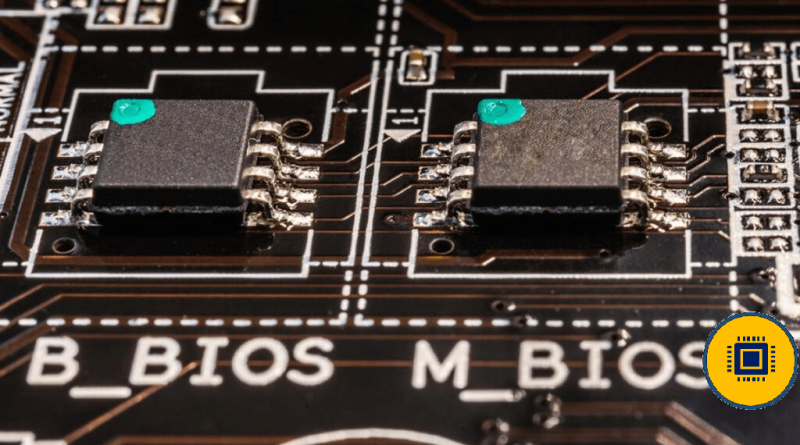
\includegraphics[scale=0.5]{Figures/BIOS}
\end{center}
\end{frame}

\begin{frame}{Núcleo o Socket}
\begin{center}
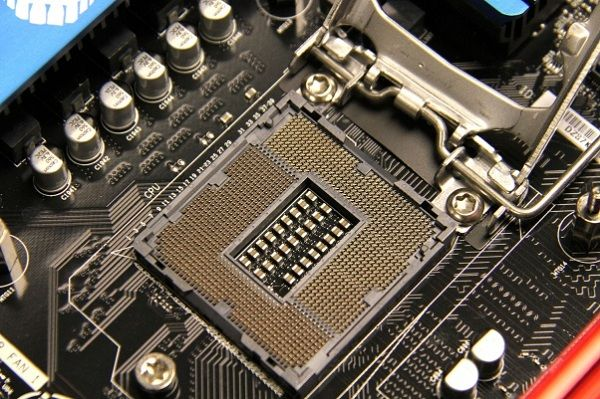
\includegraphics[scale=0.5]{Figures/Socket}
\end{center}
\end{frame}


\begin{frame}{Slots RAM}
\begin{center}
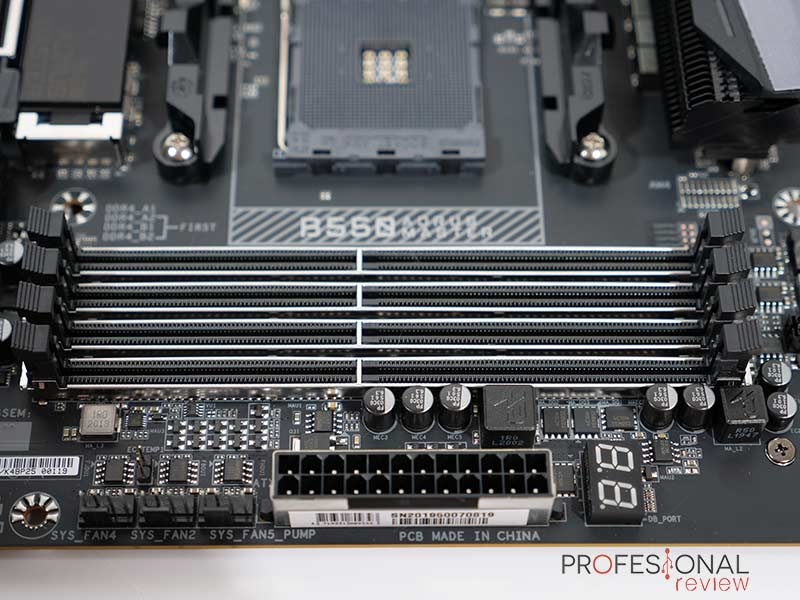
\includegraphics[scale=0.35]{Figures/SlotsRAM}
\end{center}
\end{frame}

\begin{frame}{Autopistas de datos}
\begin{center}
%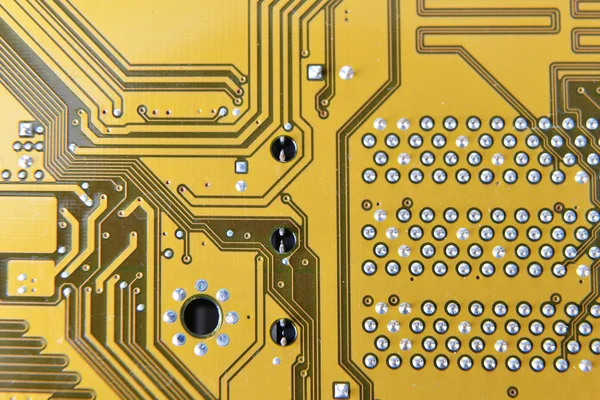
\includegraphics[scale=0.5]{Figures/BusCPU}
%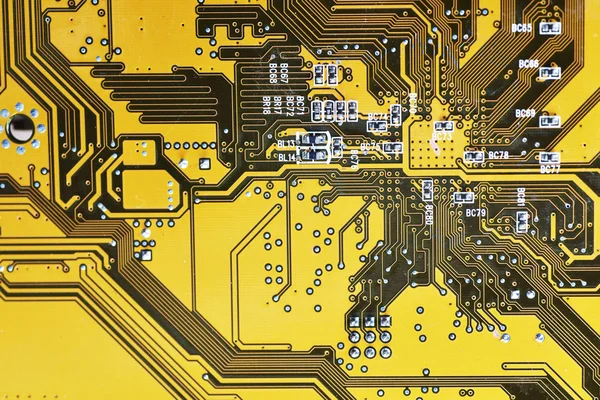
\includegraphics[scale=0.5]{Figures/BUSPlaca}
\end{center}
\end{frame}

\begin{frame}{Slot Memorias}
\begin{center}
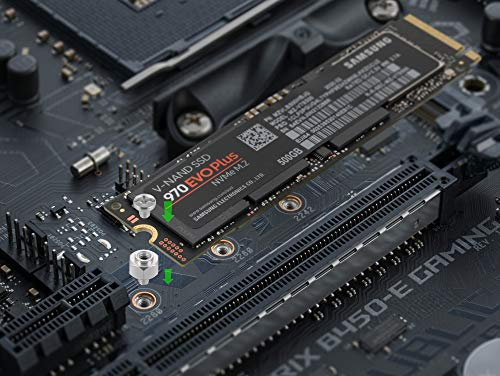
\includegraphics[scale=0.5]{Figures/SlotMemoria}
\end{center}
\end{frame}

\begin{frame}{Fuente de alimentación (PSU)}
\begin{center}
\only<1>{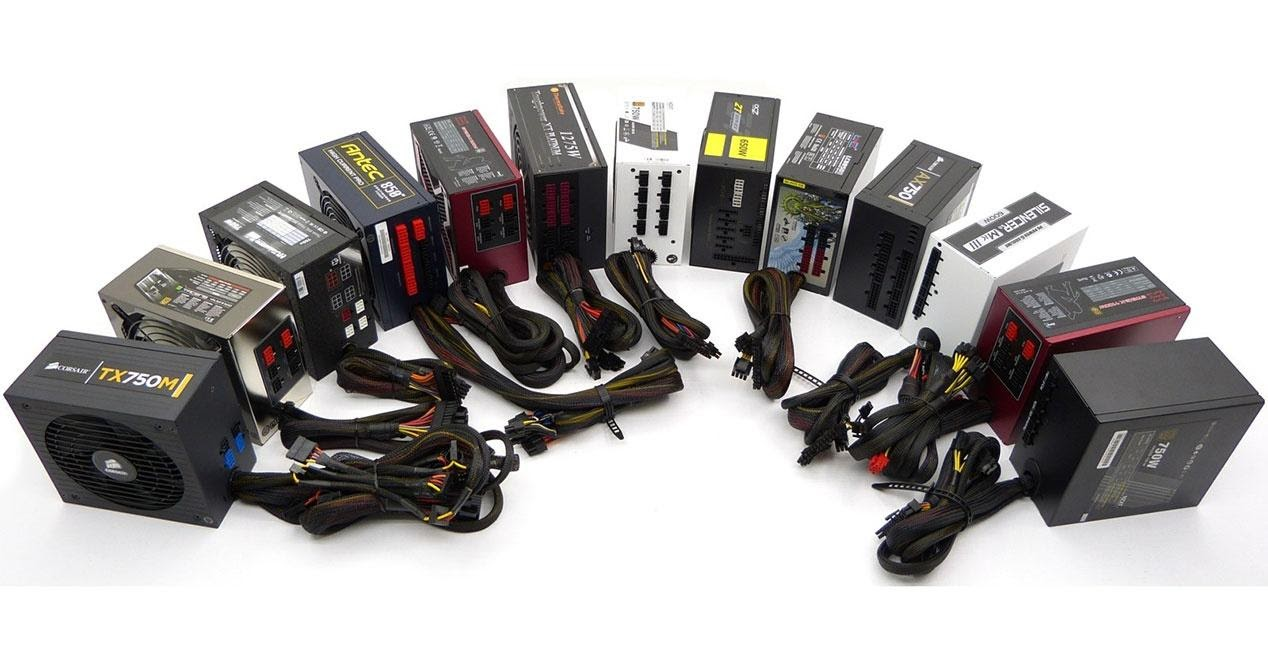
\includegraphics[scale=0.2]{Figures/Fuente}}
\only<2>{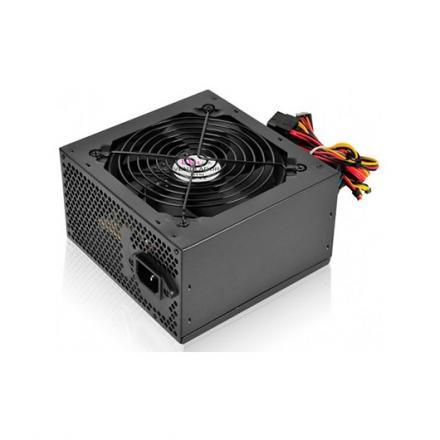
\includegraphics[scale=0.4]{Figures/Fuente1}}
\end{center}
\end{frame}


\section{Otros}
\begin{frame}
\begin{center}
\Huge{\textcolor{blue}{Otros}}
\end{center}
\end{frame}

\begin{frame}{Temperaturas}
\begin{center}
\only<1>{
\includegraphics[scale=0.7]{Figures/LeyesTermo}}
\only<2>{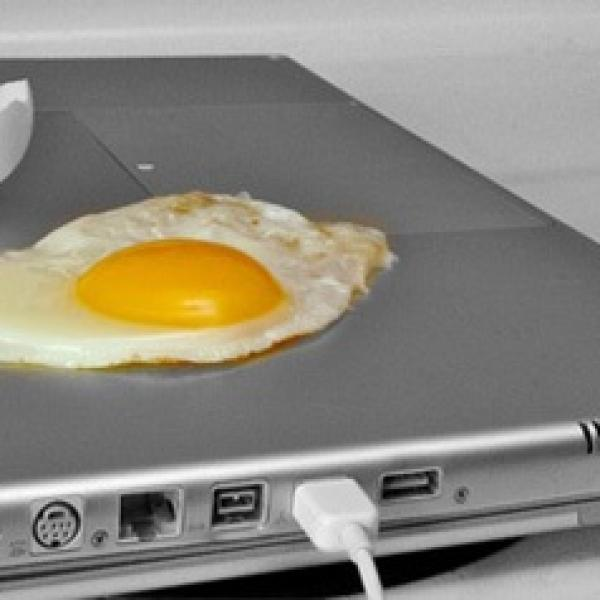
\includegraphics[scale=0.35]{Figures/Caliente}}
\only<3>{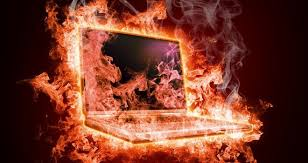
\includegraphics[scale=0.7]{Figures/Caliente1}}
\only<4>{
\includegraphics[scale=0.38]{Figures/desgracia}}
\end{center}
\end{frame}


\subsection{Enfriamiento}
\begin{frame}{Enfriamiento}
\begin{center}
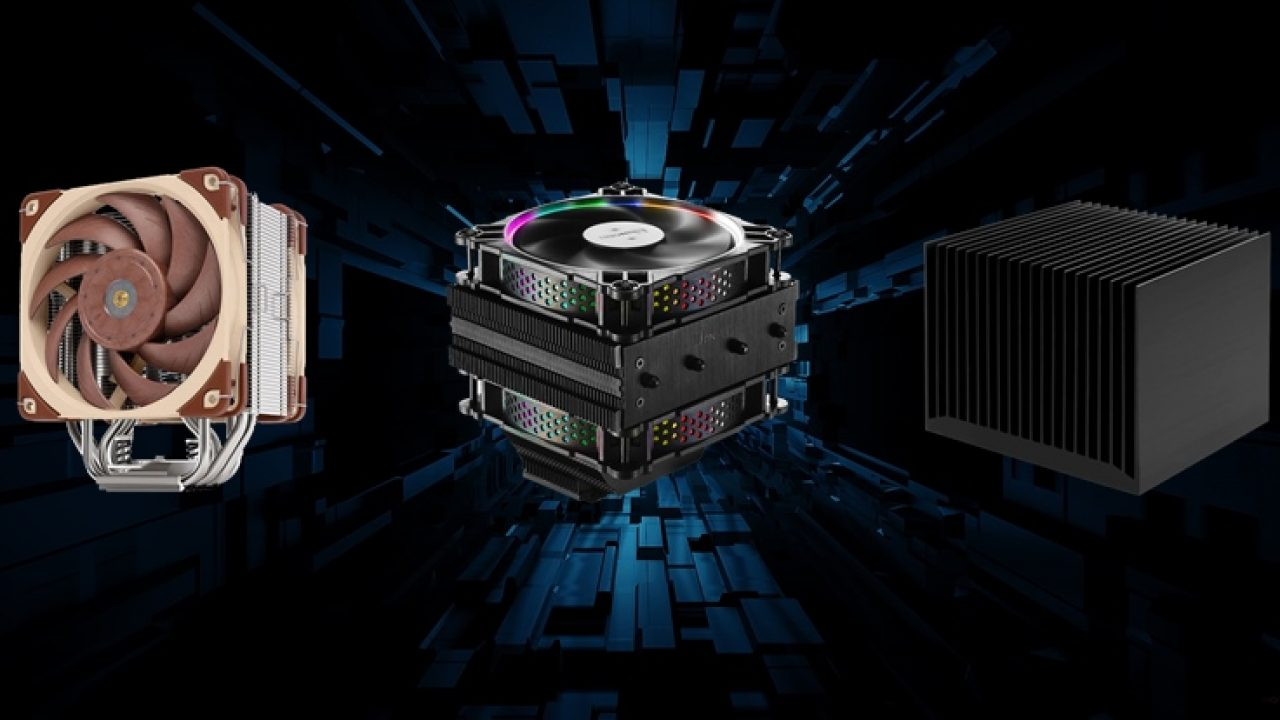
\includegraphics[scale=0.3]{Figures/disipadores}
\end{center}
\end{frame}

\begin{frame}{Disipador: Aire}
\begin{center}
\includegraphics[scale=0.5]{Figures/disipadorAire}
\end{center}
\end{frame}

\begin{frame}{Disipador: Liquido}
\begin{center}
\only<1>{\includegraphics[scale=0.4]{Figures/disipadorAgua}}
\only<2>{\includegraphics[scale=0.2]{Figures/Liquida}}
\end{center}
\end{frame}


\subsection{Chasis}
\begin{frame}{Chasis}
\begin{center}
\only<2>{\includegraphics[scale=0.35]{Figures/Chasis1}}
\only<3>{\includegraphics[scale=0.25]{Figures/ChasisCarton2}}
\only<4>{\includegraphics[scale=0.35]{Figures/ChasisCarton}}
\only<5>{\includegraphics[scale=0.25]{Figures/Chasis2}}
\only<6>{\includegraphics[scale=0.6]{Figures/Chasis}}
\end{center}
\end{frame}

\subsection{Periféricos}
\begin{frame}{Periféricos}
\begin{center}
\only<2>{\includegraphics[scale=0.2]{Figures/perifericos}}
\only<3>{\includegraphics[scale=0.3]{Figures/Perifericos}}
\only<4>{\includegraphics[scale=0.55]{Figures/perifericos1}}
\end{center}
\end{frame}

\begin{frame}{Periféricos}
\begin{center}
\includegraphics[scale=0.5]{Figures/PCH}
\end{center}
\end{frame}

\begin{frame}{Monitor}
\begin{center}
\only<1>{\includegraphics[scale=0.23]{Figures/Monitor}}
\only<2>{\includegraphics[scale=0.6]{Figures/LED}}
\only<3>{\includegraphics[scale=0.3]{Figures/rgb}}
\only<4>{\includegraphics[scale=0.5]{Figures/led1}}
\end{center}
\end{frame}

\begin{frame}{Gráficos}
\begin{center}
\only<1>{\includegraphics[scale=1.0]{Figures/DDMario}}
\only<2>{\includegraphics[scale=0.15]{Figures/SuperMarioBros}}
\only<3>{\includegraphics[scale=0.25]{Figures/DDCountry}}
\only<4>{\includegraphics[scale=0.2]{Figures/Halo}}
\only<5>{\includegraphics[scale=0.15]{Figures/Horizon-Forbidden-West-Aloy-Barba}}
\only<6>{\includegraphics[scale=0.3]{Figures/pokemon}}
\only<7>{\includegraphics[scale=0.4]{Figures/Forza}}
\only<8>{\includegraphics[scale=0.12]{Figures/TheLastOfUs}}
\only<9>{\includegraphics[scale=0.23]{Figures/zelda}}
\end{center}
\end{frame}

\subsection{GPU}
\begin{frame}{GPU Integrada}
\begin{center}
\includegraphics[scale=0.5]{Figures/ProcesadorInt}
\end{center}
\end{frame}

\begin{frame}{GPU Dedicada}
\begin{center}
\only<1>{\includegraphics[scale=0.3]{Figures/GPU}}
\only<2>{\includegraphics[scale=0.37]{Figures/GPUInt}}
\end{center}
\end{frame}

\begin{frame}
\begin{center}
\includegraphics[scale=0.3]{Figures/Milhouse}
\end{center}
\end{frame}

\begin{frame}
\begin{center}
\includegraphics[scale=0.7]{Figures/Shrek2}
\end{center}
\end{frame}

{\1
\begin{frame}[plain,noframenumbering]
  \finalpage{“homero eres tonto como una piedra y feo como una blasfemia si un extraño ofrece llevarte te subes”, Abraham Simpson  }
\end{frame}}

\end{document}